\documentclass[tikz,border=0pt,11pt]{standalone}
\usepackage[T1]{fontenc}
\usepackage[utf8]{inputenc}
\usepackage{lmodern,amsmath,amssymb}
\usepackage[swedish]{babel}
\usetikzlibrary{arrows.meta,calc,positioning,decorations.pathmorphing,decorations.pathreplacing,patterns,shadings}
\definecolor{navy}{HTML}{102F40}
\definecolor{teal}{HTML}{147D78}
\definecolor{lightteal}{HTML}{E6F1ED}
\definecolor{gold}{HTML}{B88B3B}
\definecolor{palegold}{HTML}{F7EEDB}
\definecolor{rust}{HTML}{B6533B}
\definecolor{palerust}{HTML}{FAEAE4}
\definecolor{paper}{HTML}{F7F5EE}
\definecolor{muted}{HTML}{5B6D72}
\definecolor{line}{HTML}{D6DED8}
\renewcommand{\familydefault}{\sfdefault}
\newcommand{\atom}[5]{\shade[ball color=#3!70] (#1,#2) circle (#5);\node[text=white,font=\bfseries\small] at (#1,#2){#4};}
\newcommand{\water}[3]{\begin{scope}[shift={(#1,#2)},scale=#3]\draw[navy!45,line width=2pt] (-.3,.22)--(0,0)--(.3,.22);\atom{0}{0}{rust}{O}{.22}\atom{-.3}{.22}{teal}{H}{.15}\atom{.3}{.22}{teal}{H}{.15}\end{scope}}
\newcommand{\panel}[4]{\filldraw[fill=white,draw=line,rounded corners=5pt] (#1,#2) rectangle ++(#3,#4);}
\newcommand{\note}[4]{\node[txt,text width=#3cm] at (#1,#2){#4};}
\tikzset{txt/.style={anchor=north west,align=left,text=navy,font=\small},
 head/.style={anchor=west,text=navy,font=\bfseries\large},
 label/.style={align=center,text=navy,font=\small},
 smalllabel/.style={align=center,text=muted,font=\footnotesize},
 arrow/.style={-{Latex[length=2.5mm,width=1.8mm]},line width=1.2pt,draw=teal},
 goldarrow/.style={-{Latex[length=2.5mm]},line width=1.2pt,draw=gold},
 rustarrow/.style={-{Latex[length=2.5mm]},line width=1.2pt,draw=rust},
 dashedarrow/.style={arrow,dashed},
 badge/.style={fill=lightteal,rounded corners=3pt,text=teal,font=\bfseries\small,inner sep=5pt}}
\begin{document}
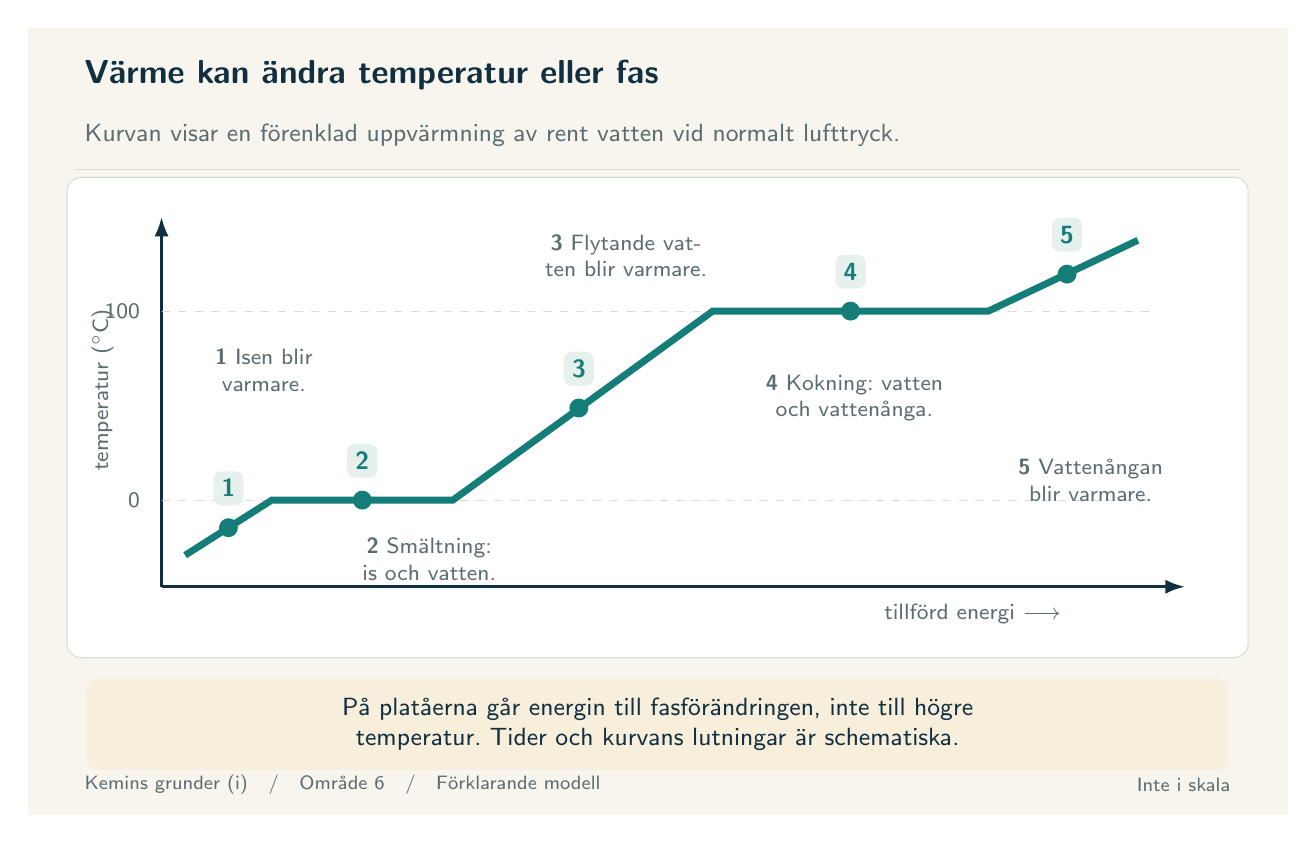
\begin{tikzpicture}[x=1cm,y=1cm]
\path[use as bounding box] (0,0) rectangle (16,10);
\fill[paper] (0,0) rectangle (16,10);
\node[head] at (.6,9.4){Värme kan ändra temperatur eller fas};
\note{.6}{8.9}{14.8}{\textcolor{muted}{Kurvan visar en förenklad uppvärmning av rent vatten vid normalt lufttryck.}}
\draw[line] (.6,8.2)--(15.4,8.2);

\panel{.5}{2}{15}{6.1}
\draw[arrow,navy] (1.7,2.9)--(14.7,2.9);\draw[arrow,navy] (1.7,2.9)--(1.7,7.6);
\node[smalllabel,rotate=90] at (.95,5.4){temperatur ($^\circ$C)};\node[smalllabel] at (12,2.55){tillförd energi $\longrightarrow$};
\draw[dashed,line] (1.7,4)--(14.3,4);\draw[dashed,line] (1.7,6.4)--(14.3,6.4);
\node[smalllabel,anchor=east] at (1.55,4){0};\node[smalllabel,anchor=east] at (1.55,6.4){100};
\draw[teal,line width=2.5pt] (2,3.3)--(3.1,4)--(5.4,4)--(8.7,6.4)--(12.2,6.4)--(14.1,7.3);
\foreach \x/\y/\n in {2.55/3.65/1,4.25/4/2,7/5.17/3,10.45/6.4/4,13.2/6.87/5}{\fill[teal] (\x,\y) circle(.12);\node[badge,inner sep=3pt] at (\x,\y+.5){\n};}
\node[smalllabel,text width=2cm] at (3,5.65){\textbf{1} Isen blir varmare.};
\node[smalllabel,text width=2.4cm] at (5.1,3.25){\textbf{2} Smältning: is och vatten.};
\node[smalllabel,text width=2.9cm] at (7.6,7.1){\textbf{3} Flytande vatten blir varmare.};
\node[smalllabel,text width=3.1cm] at (10.5,5.3){\textbf{4} Kokning: vatten och vattenånga.};
\node[smalllabel,text width=2.3cm] at (13.5,4.25){\textbf{5} Vattenångan blir varmare.};
\node[label,fill=palegold,rounded corners=4pt,inner sep=7pt,text width=14cm] at (8,1.15){På platåerna går energin till fasförändringen, inte till högre temperatur. Tider och kurvans lutningar är schematiska.};\node[anchor=west,text=muted,font=\scriptsize] at (.6,.38){Kemins grunder (i)\quad /\quad Område 6\quad /\quad Förklarande modell};
\node[anchor=east,text=muted,font=\scriptsize] at (15.4,.38){Inte i skala};
\end{tikzpicture}\end{document}
